\documentclass[crop,tikz]{standalone}

\begin{document}
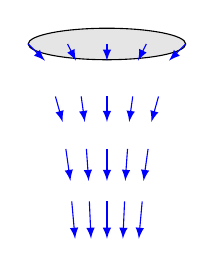
\begin{tikzpicture}
  \pgfmathsetmacro{\width}{2}; % width of opening
  \pgfmathsetmacro{\xmax}{\width/2};
  \pgfmathsetmacro{\ymax}{-0.5};
  \pgfmathsetmacro{\ymin}{-2.5};
  \pgfmathsetmacro{\nxarrows}{5}; % number of arrows in x (horizontal) direction
  \pgfmathsetmacro{\nyarrows}{4}; % number of arrows in y (vertica) direction
  \pgfmathsetmacro{\scaling}{-0.3};
  % outlet
  \draw[fill=gray!20] (0,{\ymax}) circle ({0.5*\width} and {0.1*\width});
  % boundary
  \pgfmathsetmacro{\xminboundary}{sqrt((\xmax)^2*\ymax/\ymin)};
  \draw[densely dotted,domain=\xminboundary:\xmax] plot[samples=50] function{(\xmax/x)*(\xmax/x)*\ymax};
  \draw[densely dotted,domain=-\xmax:-\xminboundary] plot[samples=50] function{(\xmax/x)*(\xmax/x)*\ymax};
  % vector field
  \foreach \NX in {1,...,{\nxarrows}} {%
    \foreach \NY in {1,...,{\nyarrows}} {%
      \pgfmathsetmacro{\Y}{\ymin + (\NY-1)/(\nyarrows-1)*(\ymax - \ymin) };
      \pgfmathsetmacro{\xminboundary}{sqrt((\xmax)^2*\ymax/\Y)};
      \pgfmathsetmacro{\X}{\xminboundary - 2*(\NX-1)/(\nxarrows-1)*\xminboundary };
      \draw[-latex,blue] ({\X}, {\Y}) -- ++ ({\scaling*\X/(2*sqrt(-\Y))}, {\scaling*sqrt(-\Y)});
    }
  }
\end{tikzpicture}
\end{document}
